\documentclass[12pt,fleqn]{article}\usepackage{../../common}
\begin{document}
Ekler

Binom ve $p$ İçin Maksimum Olurluk Tahmini [1]

$$ L(p;x) = \prod_{i=1}^n f(x_i;p) = \prod_{i=1}^n {n \choose x} p^x(1-p)^{1-x} $$

Log alalım

$$ \log L(p;x) = 
\sum_{i=1}^n \log {n \choose x} + x \log p + (1-x) \log (1-p) $$

$p$'ye göre türevi alalım, bu sırada kombinasyon ifadesi ${n \choose x}$
içinde $p$ olmadığı için o yokolacaktır,

$$ \frac{\partial \log L(p)}{\partial p} =
\frac{x}{p} - \frac{n-x}{1-p}
$$

Maksimum değeri bulmak için sıfıra eşitleyelim ve $p$ için çözelim,

$$ 0 = \frac{x}{p} - \frac{n-x}{1-p} $$

$$  \frac{x}{p} = \frac{n-x}{1-p}  $$

$$ p(n-x)  = x(1-p) $$

$$ pn - px = x-px $$

$$ pn = x $$

$$ p = \frac{x}{n} $$

Yani $p$ için maksimum olurluk tahmini $x/n$. 

Bernoulli dağılımı Binom dağılımına çok benzer, sadece onun baş kısmında
kombinasyon ifadesi yoktur. Fakat o ifade $p$'ye göre türevde nasıl olsa
yokolacağına göre Bernoulli dağılımı için de tahmin edici aynıdır.

Bayes Usulü Güven Aralığı (Confidence Intervals) 

Bayes ile bu hesabı yapmak için bir dağılımı baz almak lazım. Eğer sonuç
olarak bir tek sayı değil, bir dağılım elde edersek bu dağılım üzerinde
güvenlik hesaplarını yaparız. Mesela sonuç, sonsal dağılım (posterior) bir
Gaussian dağılım ise, bu dağılımın yüzde 95 ağırlığının nerede olduğu, ve
nasıl hesaplandığı bellidir.

Bayes Teorisi

$$ P(A \mid B)  = \frac{P(B \mid A)P(A)}{P(B)} $$

Veri analizi bağlamında diyelim ki deneyler yaparak tahmini olarak
hesaplamak (estimate) istediğimiz bir parametre var, bu bir protonun
kütlesi ya da bir ameliyat sonrası hayatta kalma oranı olabilir. Bu
durumlarda iki ayrı "olaydan" bahsetmemiz gerekir, B olayı spesifik bazı
ölçümlerin elde edilmesi "olayıdır", mesela ölçüm üç sayıdan oluşuyorsa,
biz bir ölçümde spesifik olarak $\{0.2,4,5.4\}$ değerlerini elde
etmişiz. İkinci olay bilmediğimiz parametrenin belli bir değere sahip
olması olacak. O zaman Bayes Teorisinin şu şekilde tekrar yazabiliriz, 

$$ P(parametre \mid veri ) \propto P(veri \mid parametre)P(parametre) $$

$\propto$ işareti orantılı olmak (proportional to) anlamına geliyor. Böleni
attık çünkü o bir sabit (tamamen veriye bağlı, tahmini hesaplamak
istediğimiz parametreye bağlı değil). Tabii bu durumda sol ve sağ taraf
birbirine eşit olmaz, o yüzden eşitlik yerine orantılı olmak işaretini
kullandık. Bu çerçevede "belli bir sayısal sabit çerçevesinde birbirine
eşit (equal within a numeric constant)" gibi cümleler de görülebilir. 

Örnek

Diyelim ki bir bozuk para ile 10 kere yazı-tura attık, ve sonuç altta

T H H H H T T H H H

Bu veriye bakarak paranın hileli olup olmadığını anlamaya
çalışacağız. Bayes ifadesini bu veriye göre yazalım,

$$ P(p | \{ \textrm{T H H H H T T H H H} \} \propto 
P(\{ \textrm{T H H H H T T H H H} | p) P(p) \}
$$

$P(p)$ ifadesi ne anlama gelir? Aslında bu ifadeyi $P([Dagilim] = p)$ olarak
görmek daha iyi, artık $p$ parametresini bir dağılımdan gelen bir özgün değer
olarak gördüğümüze göre, o dağılımın belli bir $p$'ye eşit olduğu zamanı
modelliyoruz burada. Her halükarda $P(p)$ dağılımını, yani onsel (prior)
olasılığı bilmiyoruz, hesaptan önce her değerin mümkün olduğunu biliyoruz, o
zaman bu onsel dağılımı düz (flat) olarak alırız, yani $P(p) = 1$.

$P(\{\textrm{T H H H H T T H H H} | p)$ ifadesi göz korkutucu olabilir, ama
buradaki her öğenin bağımsız özdeşçe dağılmış (independent identically
distributed) olduğunu görürsek, ama bu ifadeyi ayrı ayrı
$P(\{\textrm{T}|p)$ ve $P(\{\textrm{H}|p)$ çarpımları olarak
görebiliriz. $P(\{\textrm{T}|p) = p$ ve $P(\{\textrm{H}|p)=1-p$ olduğunu
biliyoruz. O zaman

$$ P(p | \{ \textrm{7 Tura, 3 Yazı} \} \propto
p^7(1-p)^3
$$

Grafiklersek, 

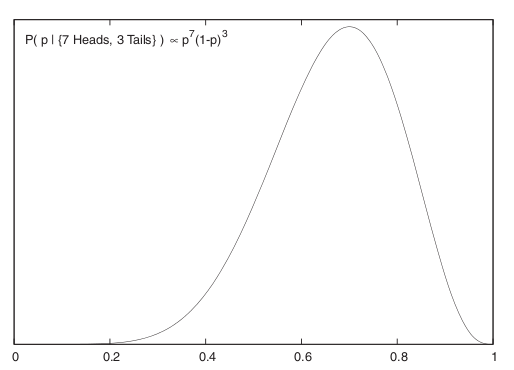
\includegraphics[height=6cm]{stat_appendix_01.png}

Böylece $p$ için bir sonsal dağılım elde ettik. Artık bu dağılımın yüzde 95
ağırlığının nerede olduğunu rahatça görebiliriz /
hesaplayabiliriz. Dağılımın tepe noktasının $p=0.7$ civarında olduğu
görülüyor. Bir dağılımla daha fazlasını yapmak ta mümkün, mesela bu
fonksiyonu $p$'ye bağlı başka bir fonksiyona karşı entegre etmek mümkün,
mesela beklentiyi bu şekilde hesaplayabiliriz.

Onsel dağılımın her noktaya eşit ağırlık veren birörnek (uniform) seçilmiş
olması, yani problemi çözmeye sıfır bilgiden başlamış olmamız, yöntemin bir
zayıflığı olarak görülmemeli. Yöntemin kuvveti elimizdeki bilgiyle başlayıp
onu net bir şekilde veri ve olurluk üzerinden sonsal tek dağılıma
götürebilmesi. Başlangıç ve sonuç arasındaki bağlantı gayet net. Fazlası da
var; ilgilendiğimiz alanı (domain) öğrendikçe, başta hiç bilmediğimiz onsel
dağılımı daha net, bilgili bir şekilde seçebiliriz ve bu sonsal dağılımı da
daha olması gereken modele daha yaklaştırabilir. 

Moment 

Olasılık matematiğinde "moment üreten işlevler" olarak adlandırılan,
başlangıçta pek yararlı gibi gözükmesede bir takım matematiksel
özellikleri olduğu için, ispatlarda oldukça işe yarayan bir kavram
vardır.

Her rasgele değişkenin bir dağılımı olduğunu biliyoruz. Her rasgele
değişkenin de ayrıca bir moment üreten fonksiyonu da vardır. Ayrıca,
moment üreten fonksiyon ile rasgele değişken arasında bire-bir olarak
bir ilişki mevcuttur. "Bu neye yarar?" diye sorulabilir; Cevap olarak,
mesela cebirsel olarak türete türete bir moment'e geldiğimiz
düşünelim, ve tekrar başka bir taraftan, başka bir formülden gene
türete türete tekrar aynı moment işlevine geliyorsak, bu demektir ki,
iki taraftan gelen rasgele değişkenler (ve tekabül eden dağılımları)
birbirine eşittir. Bazı şartlarda moment üreten işlevler ile cebir
yapmak, dağılım fonksiyonlarından daha rahat olmaktadır.

Her rasgele değişken için, moment üreten işlev şöyle bulunur.

$X$ rasgele degiskenin moment ureten operasyonu

$M(t)=E(e^{tX})$ olarak gösterilir

Ayrıksal operasyonlar için

$$ M(t) = \sum_x e^{tx}p(x) $$

Sürekli işlevler için

$$ M(t) = \int_{-\infty}^{\infty} e^{tx}f(x) \ud x   $$

Kuram

Gelelim yazımızın esas konusu olan kuramımıza.

Eğer $X_1, X_2...X_n$ bağımsız rasgele değişken ise, ve her değişkenin
$M_i(t)$ $i=1,2,3,...n$ olarak, öz olarak aynı olan birer moment üreten
işlevi var ise, o zaman,

$$ Y = \sum_{i=1}^n  aX_i $$

açılımı

$$ M_y(t) = \prod_{i=1}^n M(a_i t) $$

olacaktır. 

İspat

$$ M_y(t) = E(e^{tY}=E(e^{t(a_1X_1+a_2X_2+..+a_nX_n)} $$

$$ = E[\exp(ta_1 X_1 ta_2X_2...+ta_nX_n)] $$

$$ = E[\exp(ta_1X_1)+\exp(ta_2X_2)+ ... + \exp(ta_nX_n)] $$

$$ = E[\exp(ta_1X_1)]+E[\exp(ta_2X_2)]+ ... + E[\exp(ta_nX_n)]$$

Daha önce belirttiğimiz gibi

$$ M_i(t) = E[\exp(tX_i)] $$

olduğuna göre ve $t$ yerine $ta_i$ koyulduğunu düşünelim

$$ M_y(t) = \prod_{i=1}^n M_y(a_it) $$

olacaktır. 

Bunu $M_y(t)= (M_i(a_it))^n$ şeklinde de gösterebiliriz. 

Markov'un Eşitsizliği (Markov's Inequality)

$X$ bir negatif olmayan rasgele değişken olsun ve farz edelim ki $E(X)$
mevcut [1]. O zaman her $t > 0$ için

$$ P(X>t) \le \frac{E(X)}{t}$$

doğru olmalıdır. 

İspat

$X > 0$ olduğuna göre, 

$$ 
E(X) 
= \int_{0}^{\infty} x f(x) \ud x 
= \int_{0}^{t} x f(x) \ud x + \int_{t}^{\infty} x f(x) \ud x =
$$

$$ 
\ge \int_{t}^{\infty} x f(x) \ud x \ge t \int_{t}^{\infty} f(x) \ud x
= t P(X > t)
$$

Çebişev Eşitsizliği (Chebyshev's Inequality)

Herhangi bir $t$ değeri için, 

$$ P(|X-\mu| > t) \le \frac{\sigma^2}{t^2} $$

ve 

$$ P(|Z| \ge k) \le \frac{1}{k^2}$$

ki $Z = (X-\mu)/\sigma$, ve $E(X) = \mu$. Bunun bazı akılda kalabilecek
ilginç sonuçları $P(|Z| > 2) < 1/4$ ve $P(|Z| > 3) < 1/9$ olabilir.

İspat

Yöntem 1

Üstteki Markov'un eşitsizliğini kullanırız, oradan şu sonuca varırız, 

$$ 
P(|X-\mu| \ge t) = P(|X-\mu|^2 \ge t^2 ) \le \frac{E(X-\mu)^2}{t^2} 
= \frac{\sigma^2}{t^2}  
$$

İkinci kısım $t=k\sigma$ kullanılarak elde edilebilir.

Yöntem 2

Olasılık matematiğinde, büyük sayılar kuramı adında anılan ve olasılık
matematiğinin belkemiğini oluşturan kuramı ispatlamak için, diğer bir kuram
olan Çebişev eşitsizliğini de anlamamız gerekiyor. Çebişev eşitsizliği bir
rasgele değişken, onun ortalaması (beklentisi) ve herhangi bir sabit sayı
arasındaki üçlü arasında bir 'eşitsizlik' bağlantısı kurar, ve bu bağlantı
diğer olasılık işlemlerimizde ispat verisi olarak işimize yarar.



İspata başlayalım. Entegral ile olasılık hesabı yapmak için bize bir $x$
uzayı lazım.

$$ \mathbb{R} = {x: |x-\mu| > t} $$

Yani $\mathbb{R}$ uzayı, $x$ ile ortalamasının farkının, $t$'den büyük olduğu bütün
sayıların kümesidir.

O zaman, 

$$ P(|X-\mu| > t) = \int_R f(x) \ud x $$

Dikkat edelim $P(..)$ içindeki formül, küme tanımı ile aynı. O yüzden $P()$
hesabı ortada daha olmayan, ama varolduğu kesin bir dağılım fonksiyonu
tanımlamış da oluyor. Buna $f(x)$ deriz. $P()$'in, $f(x)$ fonksiyonunun $R$
üzerinden entegral olduğunu olasılığa giriş dersinden bilmemiz lazım. 

Eger $x \in R$ dersek o zaman

$$ \frac{|x-\mu|^2}{t^2} \ge 1 $$

t'nin denkleme bu şekilde nereden geldiği şaşkınlık yaratabilir. Daha önce
tanımlanan şu ibareye dikkat edelim, $x: |x-u| > t$ diye belirtmiştik. Bu
ifadeyi değiştirerek, yukarıdaki denkleme gelebiliriz.

Devam edersek, elimizdeki 1'den büyük bir değer var. Bu değeri kullanarak,
aşağıdaki tanımı yapmamız doğru olacaktır.

$$
\int_R f(x) \ud x \le \int_R \frac{(x-\mu)^2}{t^2}f(x) \ud x \le
\int_{-\infty}^{\infty}\frac{(x-\mu)^2}{t^2}f(x) \ud x 
$$

Ortadaki entegral niye birinci entegralden büyük? Çünkü orta entegraldeki
$f(x)dx$ ibaresinden önce gelen kısmın, her zaman 1'den büyük olacağını
belirttiğimize göre, ikinci entegralin birinciden büyük olması normaldir,
çünkü birinci entegral $f(x)$ olasılık dağılımına bağlı, entegral ise bir
alan hesabıdır ve olasılık dağılımlarının sonsuzlar arasındaki entegrali
her zaman 1 çıkar, kaldı ki üstteki $x$'in uzayını daha da daralttık.

Evet...Üçüncü entegral ispata oldukça yaklaştı aslında. Standart sapma
işaretini hala ortada göremiyoruz, fakat son entegraldeki ibare standart
sapma değerini zaten içeriyor. Önce daha önceki olasılık natematiği
bilgimize dayanarak, standart sapmanın tanımını yazıyoruz. Dikkat edelim,
bu ibare şu anki ispatımız dahilinden değil, haricinden önceki bilgimize
dayanarak geldi. Standart sapmanın tanımı şöyledir.

$$ \sigma^2 = \int_{-\infty}^{\infty} (x-\mu)^2f(x) \ud x $$

O zaman

$$
\frac{\sigma^2}{t^2}
= \int_{-\infty}^{\infty}\frac{(x-\mu)^2}{t^2}f(x)\ud x
$$

yani

$$
\int_R f(x) \ud x \le \frac{\sigma^2}{t^2} = 
\int_{-\infty}^{\infty} \frac{(x-\mu)^2}{t^2}f(x) \ud x
$$

ki $\int_R f(x) \ud x$ zaten $P(|X-\mu| > t)$ olarak tanımlanmıştı. 

Örnek

Diyelim ki bir tahmin edicimiz var, onu test etmek istiyoruz, bu bir yapay
sinir ağı (YSA) olabilir, ve elimizde $n$ tane test verisi var. Eğer tahmin
edici, yani YSA, hatalı ise $X_i=1$ olsun, haklı ise $X_i=0$ olsun. O zaman
gözlenen hata oranı (observed error rate)
$\overline{X}_n = n^{-1}\sum_{i=1}^{n} X_i$ olacaktır. Rasgele değişken
çıktılarına bakarak bunu bir $p$'si bilinmeyen bir Bernoulli dağılımından
geliyormuş gibi kabul edebileceğimizi görebiliriz. İstediğimiz gerçek -ama
bilinmeyen- $p$ hakkında irdeleme yapmak. $\overline{X}_n$'in gerçek
$p$'nin $\epsilon$ yakınında olmama olasılığı nedir?

Bernoulli'lerin özelliklerinden biliyoruz ki 

$$ V(\overline{X}_n) = V(X_1) / n = p(1-p)/n$$

Çebişev uygulayınca, 

$$ 
P(|\overline{X}_n - p| > \epsilon) \le \frac{V(\overline{X}_n)}{\epsilon^2}
= \frac{p(1-p)}{n\epsilon^2} \le \frac{1}{4n\epsilon^2}
$$

Hatırlarsak Bernoulli için $E(X)=p$. Son geçiş mümkün oldu çünkü her $p$
için $p(1-p) \le \frac{1}{4}$ olmak zorundadır. Öyle değil mi? $p(1-p)$'nin
alabileceği en büyük değer $p=1/2$ içindir, bundan farklı her $p$ değeri
$1/4$'ten küçük bir çarpım verir, mesela $p=1/3$ için
$1/3 \cdot 2/3 = 2/9$.

O zaman, ve diyelim ki $\epsilon = .2$ ve $n=100$ için $0.0625$ sınırını
elde ederiz. 

Hoeffding'in Eşitsizliği

Bu eşitsizlik Markov'un eşitsizliğine benziyor, ama daha keskin sonuçlar
verebiliyor, yani ufak güven aralıkları elde edebiliyoruz, ki bu daha fazla
kesinlik demektir. Bu eşitsizliği iki bölüm olarak vereceğiz, 

$Y_1,Y_2,..,Y_n$ bağımsız gözlemler olsunlar, ki $E(Y_i)=0$ ve
$a_i \le Y_i \le b_i$ doğru olacak şekilde. O zaman herhangi bir $t>0$ için 

1. Teori

$$ 
P \bigg( 
\sum_{i=1}^{n} Y_i \ge \epsilon \le e^{-t\epsilon} 
\prod_{i=1}^{n} e^{{t^2}(b_i-a_i)^2 / 8}
\bigg)
$$

2. Teori

$X_1,..,X_n \sim Bernoulli(p)$ olsun. O zaman herhangi bir $\epsilon > 0$ icin

$$ P(|\overline{X}_n -p| > \epsilon ) \le 2e^{-2n\epsilon^2}$$

doğru olmalıdır ki, daha önce gördüğümüz gibi,
$\overline{X}_n = n^{-1}\sum_{i=1}^{n} X_i$ olacak şekilde. 

İspat için bkz [1, sf. 67]. 

Örnek

Diyelim ki $X_1,..,X_n \sim Bernoulli(p)$. $n=100$ ve $\epsilon=.2$
olsun. Çebişev esitsizligi ile 

$$ P(|\overline{X}_n - p| > \epsilon ) \le 0.0625 $$

elde etmiştik. Hoeffding'e göre

$$ 
P(|\overline{X}_n - p| > \epsilon ) \le 2e^{-2 (100)(.2)^2} = 0.00067
$$

elde ederiz, ki bu Cebisev'den gelen $0.0625$'e göre çok daha ufak bir
değerdir.

%<a name='jensen'/>

Jensen'in Esitsizligi (Jensen's Inequality)

Teori

Eğer $g$ fonksiyonu dışbükey (convex) ise o zaman

$$
E g(X) \ge g(E(X)) 
$$

İçbukey için tam tersi geçerli.

Teorinin sözel olarak söylediği eğer $f$ fonksiyonu dışbükey ise verinin
ortalaması (beklentisi) üzerinde $f$ işletmek, o verinin $f$ değerlerinin
ortalaması ile aynı olmuyor, daha doğrusu ikinci büyüklük birinci için bir
alt sınır oluşturuyor, birinci en az ikinci kadar.

İspat

Bir $L(x) = a + bx$ çizgisi hayal edelim, bu çizgi $g(x)$'e tam $E(X)$
noktasında teğet olsun [1, sf. 66]. $g$ dışbükey olduğu için her noktada
$L(x)$ çizgisi üzerinde olması garanti,

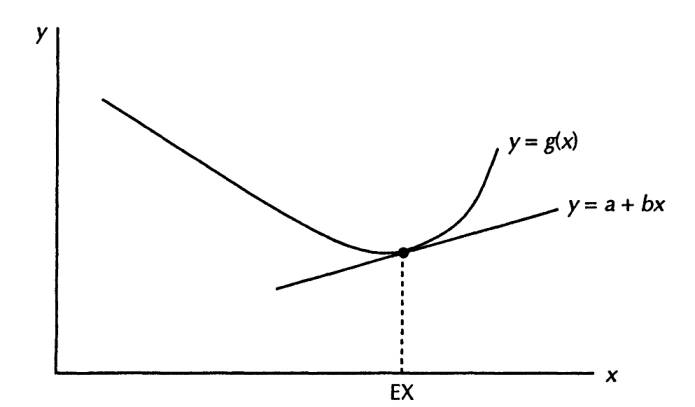
\includegraphics[width=20em]{jensen.jpg}

O zaman

$$
E(g(X)) \ge E(L(X))
$$

$E(L(X))$ formülünü açalım,

$$
E(L(X)) = E(a + bX) = a + bE(X) 
$$

Birinci geçiş basit beklenti matematiği. Son formül $L(x)$'in $E(X)$
üzerindeki formu olurdu, o zaman

$$
a + bE(X) = L(E(X))
$$

diyebiliriz.

Şimdi hatırlıyoruz ki teğet çizgi $g$ ile tam $E(X)$ noktasında kesişiyor, o
noktada değerleri aynı yani, o zaman

$$
L(E(X)) = g(E(X))
$$

Demek ki

$$
E(g(X)) \ge E(L(X)) = g(E(X))
$$

Kısaca

$$
E(g(X)) \ge  g(E(X))
$$

Teori ispatlanmış oldu.

Aslında Jensen Eşitsizliğinin daha geniş bir hali ve yorumlaması var, eğer
$g(x)$ genel olarak gayri lineer ise (sadece dışbükey değil) o zaman $g(x)$'in
ortalaması $x$ ortalamalarının üzerindeki $g$ hesabına eşit değildir [2]. Bir
alt sınır değil direk eşitsizlikten bahsediyoruz. Bu yorumlamanın da pek çok
yerde uygulaması vardır, bu ifadenin ispatı için İstatistik kaynaklarına
başvurulabilir.

Kaynaklar

[1] Wasserman, {\em All of Statistics}

[2] Denny, {\em The fallacy of the average: on the ubiquity, utility and continuing novelty of Jensen's inequality}
    \url{https://journals.biologists.com/jeb/article/220/2/139/18635/The-fallacy-of-the-average-on-the-ubiquity-utility}

\newpage

z-Tablosu

Nasıl okunur? Z-değeri -0.8994 için z kolonundan aşağı inilir, ve -0.8
bulunur, x.x9xx yani 9 için .09 kolonuna gidilir ve bu kesişmedeki değer
okunur, .1867, yuvarlanarak .19 da kabul edilebilir. 

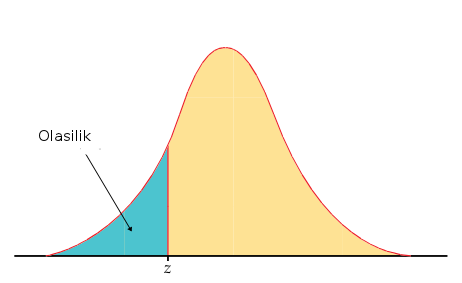
\includegraphics[height=4cm]{stat_appendix_02.png}

z \hspace{1em} .00 \hspace{1em} .01 \hspace{1em} .02 \hspace{1em} .04 \hspace{1em} .05 \hspace{1em} .06 \hspace{1em} .07 \hspace{1em} .08 \hspace{1em} .09

-3.4 .0003 .0003 .0003 .0003 .0003 .0003 .0003 .0003 .0003 .0002

-3.3 .0005 .0005 .0005 .0004 .0004 .0004 .0004 .0004 .0004 .0003

-3.2 .0007 .0007 .0006 .0006 .0006 .0006 .0006 .0005 .0005 .0005

-3.1 .0010 .0009 .0009 .0009 .0008 .0008 .0008 .0008 .0007 .0007

-3.0 .0013 .0013 .0013 .0012 .0012 .0011 .0011 .0011 .0010 .0010

-2.9 .0019 .0018 .0018 .0017 .0016 .0016 .0015 .0015 .0014 .0014

-2.8 .0026 .0025 .0024 .0023 .0023 .0022 .0021 .0021 .0020 .0019

-2.7 .0035 .0034 .0033 .0032 .0031 .0030 .0029 .0028 .0027 .0026

-2.6 .0047 .0045 .0044 .0043 .0041 .0040 .0039 .0038 .0037 .0036

-2.5 .0062 .0060 .0059 .0057 .0055 .0054 .0052 .0051 .0049 .0048

-2.4 .0082 .0080 .0078 .0075 .0073 .0071 .0069 .0068 .0066 .0064

-2.3 .0107 .0104 .0102 .0099 .0096 .0094 .0091 .0089 .0087 .0084

-2.2 .0139 .0136 .0132 .0129 .0125 .0122 .0119 .0116 .0113 .0110

-2.1 .0179 .0174 .0170 .0166 .0162 .0158 .0154 .0150 .0146 .0143

-2.0 .0228 .0222 .0217 .0212 .0207 .0202 .0197 .0192 .0188 .0183

-1.9 .0287 .0281 .0274 .0268 .0262 .0256 .0250 .0244 .0239 .0233

-1.8 .0359 .0351 .0344 .0336 .0329 .0322 .0314 .0307 .0301 .0294

-1.7 .0446 .0436 .0427 .0418 .0409 .0401 .0392 .0384 .0375 .0367

-1.6 .0548 .0537 .0526 .0516 .0505 .0495 .0485 .0475 .0465 .0455

-1.5 .0668 .0655 .0643 .0630 .0618 .0606 .0594 .0582 .0571 .0559

-1.4 .0808 .0793 .0778 .0764 .0749 .0735 .0721 .0708 .0694 .0681

-1.3 .0968 .0951 .0934 .0918 .0901 .0885 .0869 .0853 .0838 .0823

-1.2 .1151 .1131 .1112 .1093 .1075 .1056 .1038 .1020 .1003 .0985

-1.1 .1357 .1335 .1314 .1292 .1271 .1251 .1230 .1210 .1190 .1170

-1.0 .1587 .1562 .1539 .1515 .1492 .1469 .1446 .1423 .1401 .1379

-0.9 .1841 .1814 .1788 .1762 .1736 .1711 .1685 .1660 .1635 .1611

-0.8 .2119 .2090 .2061 .2033 .2005 .1977 .1949 .1922 .1894 .1867

-0.7 .2420 .2389 .2358 .2327 .2296 .2266 .2236 .2206 .2177 .2148

-0.6 .2743 .2709 .2676 .2643 .2611 .2578 .2546 .2514 .2483 .2451

-0.5 .3085 .3050 .3015 .2981 .2946 .2912 .2877 .2843 .2810 .2776

-0.4 .3446 .3409 .3372 .3336 .3300 .3264 .3228 .3192 .3156 .3121

-0.3 .3821 .3783 .3745 .3707 .3669 .3632 .3594 .3557 .3520 .3483

-0.2 .4207 .4168 .4129 .4090 .4052 .4013 .3974 .3936 .3897 .3859

-0.1 .4602 .4562 .4522 .4483 .4443 .4404 .4364 .4325 .4286 .4247

0.0 .5000 .4960 .4920 .4880 .4840 .4801 .4761 .4721 .4681 .4641

\newpage

z \hspace{1em} .00 \hspace{1em} .01 \hspace{1em} .02 \hspace{1em} .04 \hspace{1em} .05 \hspace{1em} .06 \hspace{1em} .07 \hspace{1em} .08 \hspace{1em} .09

0.0 .5000 .5040 .5080 .5120 .5160 .5199 .5239 .5279 .5319 .5359

0.1 .5398 .5438 .5478 .5517 .5557 .5596 .5636 .5675 .5714 .5753

0.2 .5793 .5832 .5871 .5910 .5948 .5987 .6026 .6064 .6103 .6141

0.3 .6179 .6217 .6255 .6293 .6331 .6368 .6406 .6443 .6480 .6517

0.4 .6554 .6591 .6628 .6664 .6700 .6736 .6772 .6808 .6844 .6879

0.5 .6915 .6950 .6985 .7019 .7054 .7088 .7123 .7157 .7190 .7224

0.6 .7257 .7291 .7324 .7357 .7389 .7422 .7454 .7486 .7517 .7549

0.7 .7580 .7611 .7642 .7673 .7704 .7734 .7764 .7794 .7823 .7852

0.8 .7881 .7910 .7939 .7967 .7995 .8023 .8051 .8078 .8106 .8133

0.9 .8159 .8186 .8212 .8238 .8264 .8289 .8315 .8340 .8365 .8389

1.0 .8413 .8438 .8461 .8485 .8508 .8531 .8554 .8577 .8599 .8621

1.1 .8643 .8665 .8686 .8708 .8729 .8749 .8770 .8790 .8810 .8830

1.2 .8849 .8869 .8888 .8907 .8925 .8944 .8962 .8980 .8997 .9015

1.3 .9032 .9049 .9066 .9082 .9099 .9115 .9131 .9147 .9162 .9177

1.4 .9192 .9207 .9222 .9236 .9251 .9265 .9279 .9292 .9306 .9319

1.5 .9332 .9345 .9357 .9370 .9382 .9394 .9406 .9418 .9429 .9441

1.6 .9452 .9463 .9474 .9484 .9495 .9505 .9515 .9525 .9535 .9545

1.7 .9554 .9564 .9573 .9582 .9591 .9599 .9608 .9616 .9625 .9633

1.8 .9641 .9649 .9656 .9664 .9671 .9678 .9686 .9693 .9699 .9706

1.9 .9713 .9719 .9726 .9732 .9738 .9744 .9750 .9756 .9761 .9767

2.0 .9772 .9778 .9783 .9788 .9793 .9798 .9803 .9808 .9812 .9817

2.1 .9821 .9826 .9830 .9834 .9838 .9842 .9846 .9850 .9854 .9857

2.2 .9861 .9864 .9868 .9871 .9875 .9878 .9881 .9884 .9887 .9890

2.3 .9893 .9896 .9898 .9901 .9904 .9906 .9909 .9911 .9913 .9916

2.4 .9918 .9920 .9922 .9925 .9927 .9929 .9931 .9932 .9934 .9936

2.5 .9938 .9940 .9941 .9943 .9945 .9946 .9948 .9949 .9951 .9952

2.6 .9953 .9955 .9956 .9957 .9959 .9960 .9961 .9962 .9963 .9964

2.7 .9965 .9966 .9967 .9968 .9969 .9970 .9971 .9972 .9973 .9974

2.8 .9974 .9975 .9976 .9977 .9977 .9978 .9979 .9979 .9980 .9981

2.9 .9981 .9982 .9982 .9983 .9984 .9984 .9985 .9985 .9986 .9986

3.0 .9987 .9987 .9987 .9988 .9988 .9989 .9989 .9989 .9990 .9990

3.1 .9990 .9991 .9991 .9991 .9992 .9992 .9992 .9992 .9993 .9993

3.2 .9993 .9993 .9994 .9994 .9994 .9994 .9994 .9995 .9995 .9995

3.3 .9995 .9995 .9995 .9996 .9996 .9996 .9996 .9996 .9996 .9997

3.4 .9997 .9997 .9997 .9997 .9997 .9997 .9997 .9997 .9997 .9998

Kaynaklar

[1] Gullickson, {\em Sociology G4075: Introduction to Social Data Analysis
  II}, \url{https://web.archive.org/web/20160312151715/http://pages.uoregon.edu/aarong/teaching/G4075_Outline/node13.html}

\end{document}



